\graphicspath{{chapters/5.Chapter_3/figures/}}

\begin{savequote}[75mm]
``All models are wrong, but some are useful''
\qauthor{- George E.P. Box \& Draper: \textit{Empirical model-building and response surfaces, 1987}}
\end{savequote}

\chapter{Metabolic integration}

\section{Introduction}

The linking of metabolism between host and endosymbiont is a fundamental 
stage in endosymbiotic integration \citep{Bhattacharya2007,Karkar2015a}.
Complementation of the respective metabolic deficiencies/limitations in
host and endosymbiont allow exploitation of novel niches and provide
the key selective benefits of endosymbiosis \citep{Hoffmeister2003}.

In order to identify putative metabolic integration it is necessary to
identify the primary ``points of contact'' between the metabolic networks 
of host and endosymbiont. These ``points of contact'' comprise two
major classes of proteins, transporters and secreted proteins. 
In the \textit{P. bursaria} systems we are mainly interested in
host and endosymbiont transporters which localise to the
perialgal vacuole (PV) membrane and the outer-membrane of the endosymbiont.
Similarly, we are interested in the host and endosymbiont proteins
which are secreted into the PV lumen. 


We can also investigate metabolic integration through the annotation and analysis
of known metabolic pathways in host and endosymbiont from the binned transcriptome
sequences.  This allows identification of pathways being expressed while
in the endosymbiotic relationship and potentially identify 
sites of metabolic integration between host and endosymbiont e.g. \citep{Russell2013}.


%By identifying these networks via the annotation and analysis of
%assembled host and endosymbiont transcript complements it is putatively
%possible to identify direct pathway integration.  For example,
%the completion of a particular pathway via proteins derived from both
%host and endosymbiont.

%Furthermore, comparison of networks derived from endosymbiotic
%species to previously sequenced genomes of 
%
%networks to 
%previously sequenced genomes from relatives of host and endosymbiont 
%such as \textit{P. caudatum} 
%and \textit{M. pusilum} NC64A can
%be used to identify possibly 

Finally, a characterisation of metabolites present in the system can be used
to further interrogate host and endosymbiont metabolic function.  A metabolomics
based-approach has the benefit of directly characterising the metabolites
themselves and thus determining biological activity at the top functional level.
Therefore, relative to analyses relying on abstracted measures such as 
transcription levels or gene copy number, novel information about cellular dynamics
can be revealed. This is particularly important in cases of 
of cryptic regulatory systems that break-down direct mapping from genes to 
transcripts to proteins to metabolites. 
By using both targeted and untargeted metabolomics approaches 
it is possible to survey the combined
pool of host and endosymbiont metabolites both qualitatively and quantitatively. 
These inferences can then be correlated with other data such as the
presence of transcripts involved in the synthesis or degradation of these metabolites. 

By utilising these three separate streams of metabolic analysis: comparative transcript annotation
and mapping, directed identification and analysis of transporters and secreted
proteins and metabolomics, we maximise the strength of any inferences and 
reduce the chance of false negatives.
First, I will summarise what is currently known about the metabolic
integration of \textit{P. bursaria} and its green algal endosymbionts before
discussing each of the analytical approaches that will be taken in more detail.


\subsection{Metabolism of host and endosymbiont}

The most obvious point of metabolic integration in any endosymbiosis
featuring a photosynthetic partner is that of the flow of photosynthates
from endosymbiont to host.
This is believed to primarily be in the form of carbohydrates such as maltose \citep{Muscatine1967}.
In return, the host facilitates increased rates of photosynthesis in the endosymbiont \citep{Sommaruga2009},
via supply of \(CO_{2}\) \citep{Parker1926}, one or several forms of nitrogen \citep{Johnson2011},
and mono- and divalent cations such as \(K^{+}\), \(Mg^{2+}\), and \(Ca^{2+}\). 
All of which have key roles in photosynthesis \citep{Kato2009a}.

%\subsubsection{Carbohydrate Metabolism}
%Since their discovery \citep{Cohen1957}, several functional types of transporter proteins have been identified:
%uniporters which facilitate transfer along the sugar gradient (e.g. hexose
%transporter (HXT), glucose-transporter (GLUTs), and SWEETs),
%and cotransporters which couple transport to another gradient. 
%Co-transporters are further divided into symporters such as sodium-glucose symporters (SGLTs), sucrose-\(H^{+}\) 
%cotransporter (STP), and SUT which co-transport cations in the same direction and
%antiporters such as the tonoplast sugar transporter (TST) that uses opposing
%gradients \citep{Chen2015}.

\subsubsection{Photosynthate}
The transfer of maltose, glucose, fructose and malate from endosymbiont
to host has been observed previously using radiolabelling e.g.
\citep{Brown1974}.  Furthermore, green algae strains competent to
form endosymbioses can be induced (via modifying pH) to release significantly
more photosynthate (in the form of \(\sim 95\%\) maltose) than strictly free-living strains
(on the order of \(5.4-86.7\%\) vs. \(0.4-7.6\%\)
of total photosynthate) \citep{Muscatine1967a}.
Interestingly, the export of photosynthate from the PV to the host cytoplasm may be dependent on a transporter
derived from the \textit{C. variabilis} 1N in the \textit{P. bursaria} Yad1g endosymbiosis \citep{Kodama2008}.

In terms of the uptake of saccharides,
\textit{C. variabilis} F36-ZK endosymbiont strains
seem incapable of directly utilising sucrose, maltose, glucose or fructose in free-living culture \citep{Kamako2005,Kato2009a}.
Glucose, does promote growth however, via an apparent sensing pathway that leads to the up-regulation
of amino acid importers \citep{Kato2009a}.
On the other hand, the free-living \textit{C. vulgaris} strains have an inducible 
system for active hexose uptake \citep{Tanner1974}.
In order of highest to lowest uptake rate, the free-living \textit{C. vulgaris} 
took up sucrose, glucose and maltose but not fructose \citep{Kato2009a}.


\subsubsection{Nitrogen}
Nitrogen is the most transferred material between host and endosymbiont
after carbon \citep{Kato2009a}.  There has been considerable research and interest
in exactly what form this nitrogen exchange takes \citep{Kato2006,Kamako2005,McAuley1986}.

\textit{C. variabilis} (both NC64A and the Japanese F36-ZK) have been 
found to be able to use amino acids effectively as a nitrogen source but
only minimally utilise ammonium (\(NH_4^{+}\)) and are incapable of effective
nitrate (\(NO_3^{-}\)) or nitrite (\(NO_2^{-}\)) use \citep{Kamako2005,Kato2009a}.
Similar patterns have been observed in \textit{M. reisseri}, although
all strains tested could utilise nitrate and 3/4 could use nitrite
to greater or lesser degrees \citep{Kessler1990}.
%As for the other two species of green algal \textit{P. bursaria} endosymbionts,
%\textit{Coccomyxa} sp. and \textit{C. vulgaris}, \textit{Coccomyxa} 
%can likely utilise nitrate \citep{Sanz-Luque2015}
On the other hand, free-living species such as \textit{Parachlorella
kessleri} can effectively utilise all of the nitrogen sources mentioned \citep{Kato2009a} 
(although amino acid utilisation has to be induced with glucose treatment 
\citep{Cho1981}).


In terms of amino acids as a nitrogen source there isn't
a high degree of correlation between the ability to uptake an amino acid
and its usage \citep{Kato2009a}.
For example, while \textit{C. variabilis} F36-ZK can
uptake all 20 amino acids, only 6 (L-arginine, L-asparagine,
L-glutamine, L-serine, L-alanine) were found to promote growth \citep{Kato2006}.
This was despite some of these 6 being taken up at lower rates
than some non-utilised amino acids such as L-proline, L-cysteine or L-leucine \citep{Kato2006}.

Similarly, \textit{C. variabilis} NC64A was found to have stimulated growth
in the presence of L-arginine and L-glutamine, whereas another \textit{C. variabilis}
strain, 3N813A, used every amino acid apart from L-lysine and L-glutamic acid \citep{McAuley1986,Kato2009a}.

%Glutamine synthetase likely plays a role in the endosymbiotic utilisation
%of amino acids that can be broken down to generate intracellular ammonium
%after uptake \citep{Rees1995,Kato2009a}.
%
%There is also evidence that the expression of this protein is light-dependent
%in \textit{C. variabilis} \citep{Kato2006}.
The free-living \textit{C. vulgaris} NIES-227 was found to not utilise
any amino acid apart from low levels of uptake of L-arginine \citep{Kato2006}.
Therefore, even within the \textit{C. variabilis} strains there is a range 
of traits in terms of amino acid uptake and utilisation.


Kinetic analyses and competitive assays indicate three amino acid transport
systems in \textit{C. variabilis} F36-ZK, a general amino acid tranporter
for all amino acids except L-alanine, a basic transporter for L-arginine and L-lysine
and a specialised L-alanine transporter \citep{Kato2009b,Kato2009a}.
All of these are constitutively functioning, active, amino-acid symporters \citep{Kato2009b,Kato2009a}.

%Although glucose did increase the rate of amino acid uptake by some partially defined sensing system
%and resorted uptake in the casoe of calcium ihibtion \citep{Kato2008,Kato2009a}.
%
% (although glucose and maltose
%did stimulate growth \citep{Kamako2005} it was via a mechanism which promoted increased uptake of a nitrogen source
%\citep{Kato2009a}).

As \textit{P. bursaria} cannot import nitrate \citep{Albers1982} the heterogeneous
loss of nitrate and nitrite utilisation in several endosymbiotic strains 
is perhaps not surprising \citep{Kato2009a}.
Without host nitrate uptake there is no pressure to maintain enzymes 
necessary for this pathway as an endosymbiont.
This reduced selection pressure for nitrate and nitrite utilisation 
may explain the presence of low-activity mutant Nitrate Reductase (NR) and Nitrite
Reductase (NiR) in the two \textit{C. variabilis} strains \citep{Kato2009a}. 

%On the other hand in free-living organisms utilisation of the usually rare
%inorganic sources of nitrogen
%such as ammonium, nitrate and nitrite often a major limit on growth and productivity 
%\citep{Giordano2014}.
%Constitutive expression is another adapation to endosymbiosis and metabolic integration as
%the free-living \textit{C. vulgaris} strains tested must have induced expression of these
%transporters \citep{Cho1981}.
% Respiration of the host plays a role in the gas exchange of \(CO_2\) and \(O_2\) 
% to the endosymbiont, with the algae displaying higher levels of photosynthetic
% activity while in association with the host due to the increase host related 
% \(CO_2\) respiration \citep{Reisser1980}.
%Addition of glucose, which likely increases host respiration rate and thus \(CO_2\)
%evolution increases the rate of photosynthetic oxygen production commensurately \citep{Reisser1980}

%In \textit{Parachlorella kessleri} (previous \textit{Chlorella kessleri} \citep{Krienitz2004,Hoshina2010})
%
%Chlorella \(H^{+}\)-monosaccharide (HUP1) co-transporters \citep{Sauer1989}
%have been identified (via hexose-transport deficient mutant screens \citep{Sauer1986}
%and localised to the plasma membrane \citep{Stadler1995}
%Additionally these transporters have been identified in the
%\textit{Auxenochlorella protothecoides} (formerly \textit{Chlorella protothecoides} \citep{Champenois2014}) genome \citep{Gao2014}.

\subsubsection{Cations}
The final major group of host-endosymbiont transferred metabolites
are those of mono- and divalent cations.  Specifically
\(Ca^{2+}\), \(Mg^{2+}\) and \(K^{+}\) \citep{Kato2009a}.  All of 
these have key roles in photosynthesis.
Interestingly, \(Ca^{2+}\) has also been found to inhibit amino acid uptake \citep{Kato2008}.
As glucose has been found to increase amino acid uptake, some researchers
have hypothesised that the relative concentration of photosynthates
and \(Ca^{2+}\) in the PV lumen defines a photosynthate-amino acid
barter system between endosymbiont and host \citep{Kato2009a}.

\subsection{Identifying direct points of contact}

\subsubsection{Transporter proteins}

The most important group of proteins in the control and evolution
of metabolic integration is that of host and endosymbiont transporter proteins.
This is due to their role in facilitating diffusion and active transport
across the lipid membranes that exist between host and endosymbiont.
%While the role of transporters have been investigated extensively in 
%several symbioses, these typically focus on organellar endosymbionts where
%metabolic co-dependence has become fixed \citep{Yuan1994,Tyra2007,Huang2007,Li2010a} 
%or ecological community interactions 
%\citep{Richards2013,Hirner2006,Bachmann2013,Oldroyd2009}.

Without transporters many metabolically important 
large uncharged polar molecules (e.g. carbohydrates, amino acids)
and charged molecules (e.g. the various biologically relevant cations and anions such
as \(H^{+}\)) are incapable of significant rates of diffusion 
across membranes even in the presence of high concentration gradients. 
Therefore, the presence of transporters is vital to facilitating
any interaction involving these groups of metabolites. 


Several metabolites are, however, capable 
of unfacilitated diffusion across lipid membranes at significant rates.
These include important respiratory gases such as \(O_{2}\) and \(CO_2\),
hydrophobic compounds like benzene and small uncharged polar molecules
(e.g. \(H_2O\) and ethanol) \citep{cooper2013the,alberts2015molecular}.  
Despite this, transporter proteins have evolved to facilitate
even more rapid diffusion of some of these metabolites e.g. aquaporins
\citep{Agre1993}.  


Finally, certain transporters can provide the ability
to actively transport metabolites against concentration gradients. 
This involves the expenditure of energy (typically in the form of ATP)
to directly pump compounds or generate an opposing gradient which can be
exploited (primary vs secondary active transport). 

\noindent There are 5 functional groups of transporters \citep{Saier2014}:
\begin{itemize}
    \item Channel/Pore types which catalyse diffusion of metabolites along concentration
        gradients e.g. porins and the Mitochondria and Plastid Porin (MPP) family.
    \item Electrochemical Potential-driven transporters which use a carrier-mediated process to catalyse
        uniportation (single metabolite) or cotransportation (two species in the same
        direction, symportation, or two species in opposite direction, antiportation).  These make use
        of chemiosmotic gradients but generally do not directly make use of cellular energy molecules
        such as ATP. However, many make use of a gradient/potential generated by the active transport
        of solutes by another complex, in this case they can referred to as secondary active transporters.
        Electrochemical Potential-driven transporters are a very large family and include 
        the ubiquitous major facilitator superfamily (MFS) and Cation Diffusion Facilitator (CDF) families. 
    \item Primary active transporters which use a direct source of chemical, electrical or light energy 
        such as ATP, voltage or photon to drive transport against concentration gradients.  Transporters
         of this type form many of the components fundamental to life as they allow an organism to 
         decouple itself directly from environmental and intracellular gradients. 
         They include rhodopsins, ATP-binding Cassette (ABC) Superfamily, and the general Secretory Pathway (Sec)
        family.
    \item Group translocators, which modify a substrate during transportation e.g. polysaccharide synthesis
        during secretion in the Polysaccharide Synthase/Exporter family and the Fatty Acid Group Translocation (FAT)
        family which can acylate fatty acids during transport.
    \item Transmembrane Electron Carriers which transport single electrons from a donor to an acceptor across
        a membrane. The major groups of these include the cytochrome and Photosystem I complexes. 
\end{itemize}

This analysis will focus on transporters of the first 4 classes.
In the case of \textit{P. bursaria} and its endosymbiont we are
particularly interested in 
the transporters of the host perialgal vacuole membrane and those of the outer membrane of the green
algal endosymbiont.

Therefore, the first step to the successful analysis of the metabolic
integration of host and endosymbiont is the accurate identification of
transporter proteins present in their respective binned transcriptome
sequences.   By both identifying these proteins 
and qualitatively investigating their day:night expression,
targets can be generated for further analysis.  
Specifically, validation of function and 
analysis of localisation to the PV and/or algal outer
membrane.  

%The importance of these systems in metabolic integration is further 
%evidenced by the the way the evolution of protein import systems 
%from host to endosymbiont, such as the TICs/TOCs and TIMs/TOMs
%of plastids and mitochondria, is considered by many 
%to be the main constraint in the establishment of an endosymbiont
%as an organelle \citep{Pfanner2001.Keeling2008a}.

Transporter proteins can be identified
primarily via annotation of transmembrane (TM) domain motifs
and homology searches to previously
identified transporters \citep{Saier2006,Saier2009,Saier2014}.
All transporters feature at least 1 TM helix, usually considerably
more \citep{VonHeijne2006}.  However, as not necessarily every sub-unit of
a transporter will contain a TM domain and as our assemblies consist of 
numerous partial transcripts
it is necessary to not rely exclusively on TM prediction to discover
transporter proteins.

%One obvious target of such is the sugar and amino acid transporters which facilitate the
%secretion and uptake of photosynthate and amino acid between host and endosymbiont.

\subsubsection{Secreted proteins}

The next major class of proteins involved in endosymbiosis
are those which are secreted in the PV lumen. 
Host and endosymbiont derived proteins targeted to the lumen of
this vacuole are responsible for generating the local environment
for endosymbiosis.  This is fundamental to the exchange of metabolites
between host and endosymbiont as this is the cellular context 
in which that exchange must occur.  Furthermore, in the establishment
of endosymbiosis secreted effectors from the endosymbiont
are likely responsible for the modification of a phagosomal vesicle into 
the perialgal vacuole. 

One particularly interesting example to identify would be the 
hypothesised endosymbiont derived transporter exported
to the PV membrane that is responsible for export
of photosynthate to the host cytoplasm \citep{Kodama2008}.

%Identification of secreted proteins also offers
%a chance to further elucidate the function of novel or poorly 
%characterised transporters that have been identified. 
%For example, 

The identification of secreted proteins relies on the analysis
of signal peptides and/or a range of standard classification
algorithms based on sequence and compositional features.   
Signal peptides are short 15-30 amino acid N-terminal sequences
that determine targeting of proteins to cellular compartments
\citep{Schatz1996,Rusch1995}.

SignalP \citep{Nielsen1997} has proven the most effective method of predicting
the presence of signal peptides \citep{Lee2009a,Petersen2011}.
This method uses a standard feed-forward artificial neural network
with 8-41 hidden units (depending on whether the organism is eukaryotic, 
gram positive or gram negative) trained with back-propagation.

Subcellular localisation of a given protein can also be inferred
using tools such as the WoLF PSORT \citep{Horton2007a}.
This tool implements a standard \(k\)-neighbours classifier
trained on localisation labelled proteins from SwissProt 
and uses PSORTII \citep{Nakai1992,Nakai1999,Horton1997} and iPSORT \citep{Bannai2002} 
derived sequence features and automatic inference of weightings \citep{Horton2006}. 

In addition to these tools, there are many other systems that have been
designed to predict protein localisation.  In order to maximise
the probability of successful identification of secreted proteins I have
created a consensus ensemble classifier that incorporates predictions from 
several of these tools, principally SignalP, TMHMM, TargetP, ChloroP, and WoLFPSort. 
%
%Secreted proteins can be effectively identified by 
%searching for the presence of N-terminal signal peptides. 
%
%These are short 15-30 amino acid N-terminal sequences cleaved during translocation.
%They aren't conserved sequences but are present across the tree of life.
%
%Feature a biochemical compositional fingerprint 
%of positively charged residues, hydrophobic residues and polar uncharged
%residues with distinctive points before site.l \citep{Emanuelsson2007}
%

\subsection{Metabolic mapping}

Metabolic pathways form the functional backbone of all biological processes. 
The Kyoto Encyclopedia of Genes and Genomes (KEGG) \citep{Ogata1999,Okuda2008,Kanehisa2014} 
and MetaCyc \citep{Caspi2007} databases form an important resource for contextualising
genomic and transcriptomic scale results into these networks. 
The utility of this approach is emphasised by the presence of numerous
tools and analytical pipelines to explore these databases 
e.g. \citep{Okuda2008,Nakao1999,Karp2002,Karp2010,Antonov2008,Klukas2007}.

By comparing the relatively complete predicted peptides sets from 
the sequenced endosymbiotic algae \textit{C. variabilis} NC64A and \textit{Coccomyxa
subellipsoidea} C-169 genome projects to the predicted endosymbiont binned peptides
from the transcriptomes of \textit{M. reisseri} and \textit{C. variabilis} 1N
it is possible to infer which endosymbiotic metabolic pathways 
are active in the latter two endosymbionts.  Furthermore, identification
of pathways unique to individual algae can identify potential distinct
adaptations to endosymbiosis in that algae.

%\subsection{Metabolomics}
%
%A pilot untargeted global metabolomic profile was generated
%for \textit{P. bursaria}-\textit{M. reissieri} CCAP 1660/12 
%culture to test the feasability of this approach and help optimise
%chromatography and 
%
%Finally, a proof of concept for the targeted metabolomic
%analysis of this system was conducted used HPLC-QQQ
%to determine the relative abundances of amino acids
%in the culture between day and night conditions. 
%
%In the case of \textit{P. bursaria} and its green algal endosymbionts 
%there are
%
%
%\subsubsection{Untargeted Global Profiling}
%GCMS, LCMS,
%
%\subsubsection{Targeted Analysis of Key Classes of Compounds}
%
%Mass spectrometry also offers methods by which a targeted 
%analysis of key classes of compounds can be conducted. 
%
%
%While few
%Amino acids 


\section{Aims}

The principal aim of this chapter is to identify
likely points of metabolic integration between host and 
endosymbiont to generate targets for subsequent 
targeted mass spectrometry, RNAi and qPCR based validation
experiments. 
This will be achieved by:
\begin{itemize}
\item Identifying
    transporter proteins present in the endosymbiont
    binned transcripts from the CCAP1660/12 RNAseq analysis
    and analysing them for qualitative 
    expression across day and night. 
\item Identifying
    secreted proteins present in the endosymbiont
    binned transcripts from the CCAP1660/12 RNAseq analysis
    and analysing them for qualitative 
    expression over day and night. 
\item Comparative analysis of metabolic pathways 
    between host and endosymbiont relative to 
    sequenced green algal genomes. 
\item A pilot untargeted global metabolomic profile of the 
    system and comparison of day to night.
\item Targeted quantitative analysis of amino acid concentrations
    between day and night. 
\end{itemize}

\section{Methods}

\subsection{Transporter analysis} 

\subsubsection{Transporter identification pipeline}

Transporters were identified in the 4 sets of sequences (\textit{C. variabilis}, \textit{M. reisseri},
\textit{C. vulgaris} and \textit{C. subellipsoidea}) using the following set of pipe-lined filters:
\begin{enumerate}
    \item Transmembrane (TM) domains were predicted for each sequence using an HMM approach implemented 
        as part of TMHMM2 \citep{Sonnhammer1998,Krogh2001}
and sequences predicted to contain at least 1 TM domain were extracted.
    \item These sequences were then used to search a PFAM database of profile HMMs \citep{Eddy1995} 
        via HMMER3's hmmscan utility \citep{Eddy1995,Johnson2010,Eddy2011,Mistry2013}
        and sequences with a hit to a PFAM domain at an independent e-value of \(1e^{-5}\) were retained.
    \item These hits were then finally filtered for PFAM domains which mapped to transporter 
        families classified by the Transporter Classification Database (TCDB) \citep{Saier2006,Saier2009,Saier2014}
        mapping files.
\end{enumerate}

Additionally, to ensure thorough discovery of 
all \textit{M. reisseri} transporters, \textit{M. reisseri} binned sequences 
were BLASTP-ed against the nr protein database with an e-value of \(1e^{-3}\) and 
a maximum of 20 hits.
InterproScan \citep{Zdobnov2001a} was then used to 
further annotate these proteins incorporating
results from BlasProDom \citep{Servant2002}, FPrintScan \citep{Attwood1994}, 
HMMER \citep{Mistry2013} scans against the PIR \citep{Barker1998}, PFAM \citep{Bateman2002}, 
SMART \citep{Schultz1998}, PANTHER \citep{Thomas2003a} and TIGRFAM databases \citep{Haft2003}, 
ProfileScan \citep{Gribskov1988},
HAMAP \citep{Lima2009}, PatterScan, 
SuperFamily \citep{Gough2002}, 
SignalP \citep{Petersen2011}, TMHMM \citep{Sonnhammer1998}, 
Gene3D \citep{Buchan2002}, Phobius \citep{Kall2007}
and Coils. Results were then mapped to GO terms \citep{Ashburner2000,Harris2004}
and annotated via BLAST2GO \citep{Conesa2005a}.

Finally, all proteins annotated to have a GO term associated with ``transport'' and
``transport activity'' (specifically \texttt{GO:0006810} and its child
terms) were extracted.  

This set was then filtered for the presence of TM domains and to remove
organelle related transporters such as cytochrome system and photosystems
as these are unlikely to localise anywhere other than the mitochondria
and chloroplast.

\subsection{Secretome prediction}
A conservative set of secreted proteins were predicted 
using the following consensus ensemble classifier:
\begin{enumerate}
    \item Signal peptides were detected using SignalP4.1 and mature sequences
        created for each sequence with a signal peptide
    \item Sequences detected to have a TM domain (by TMHMM) within either the mature sequence or 
        full length for proteins without signal peptides were discarded.
    \item Signal peptides were re-added to mature sequences and the 
        remaining sequences were then filtered using for those predicted as secreted by TargetP1.1 
    \item These sequences were then filtered down to those which had extracellular
        localisation in WoLFPSORT 0.2 
    \item Finally, for the endosymbiont, secreted protein found to have a Chloroplast
        targeting signal (via ChloroP1.1) were removed.
\end{enumerate}

In addition to this, a larger permissive set was generated without the TMHMM filtering 
step and retaining all proteins predicted to be extracellular or have a signal
peptide targeting for secretion.

\subsection{Qualitative expression analysis}

Kallisto \citep{Bray2015} was used to pseudoalign and estimate abundances for 
all taxonomically screened single cell 
libraries (4 dark and 3 light) to the called ``endosymbiont''
binned CDS sequences from the \textit{P. bursaria} CCAP 1660/12
transcriptome (see Chapter 4).

Kallisto doesn't align reads to references in the same
manner as conventional short read alignment algorithms
such as Bowtie2 \citep{Langmead2012}.  Instead of specifically 
mapping a read to a set of co-ordinates it instead
determines which transcripts are compatible with the alignment 
of a given read.  This is achieved via decomposition of transcripts
in de-Bruijn graphs and fast \(k\)-mer hashing to compare reads to transcript
graph nodes in constant time.  These \(k\)-compatibility classes are then used with
bootstrapped expectation-maximisation to estimate transcript quantification and
determine uncertainty \citep{Bray2015}. 

Results were visualised and analysed using ``sleuth'' and the
seaborn plotting library \citep{michael_waskom_2015_19108}.

\subsection{Metabolic mapping analysis}

First, predicted proteomes were obtained or generated for
\textit{Coccomyxa subellipsoidea} C-169, \textit{Chlorella variabilis}
NC64A, \textit{Chlorella variabilis} 1N, and \textit{M. reisseri}. 

For \textit{M. reisseri} the endosymbiont binned sequences from the transcriptomic
sequencing project discussed in the previous chapter were used. 
\textit{Coccomyxa subellipsoidea} C-169 genome project \citep{Blanc2012} version 2.0 
JGI annotated proteins (created 12-01-2014) were downloaded from JGI's
Phyotozome v10.3.1 \citep{Goodstein2012}. 
Similarly, the ``best'' annotated proteins from
version 1 of the \textit{Chlorella variabilis} NC64A genome project \citep{Blanc2010}
were downloaded from JGI's genome portal \citep{Grigoriev2011,Nordberg2014}

However, to obtain \textit{C. variabilis} 1N endosymbiont peptides 
a reassembly and binning of raw sequencing data from \citep{Kodama2014}
was conducted (discussed below). 

Once all sequences were acquired they were annotated using KEGG
orthology.  This was achieved 
using the KEGG Automatic Annotation Server (KAAS) \citep{Moriya2007a}
single-directional best hit with both BLAST and GHOSTZ \citep{Suzuki2014,Suzuki2015} 
method against the following 40 gene sets: \textit{Homo sapiens}, 
\textit{Drosophila melanogaster}, \textit{Caenorhabditis elegans},
\textit{Arabidopsis thaliana}, \textit{Gylcine max},
\textit{Vitis vinifera}, \textit{Oryza sativa}, 
\textit{Ostreococcous lucimarinus}, \textit{Ostreococcus tauri},
\textit{Micromonas} sp. RCC299, \textit{Cyanidioschyzon merolae},
\textit{Galdieria sulphuraria}, \textit{Saccharomyces cerevisiae},
\textit{Candida albicans}, \textit{Neurospora crassa}, \textit{Aspergillus nidulans},
\textit{Coccidioides immitis}, \textit{Schizosaccharomyces pombe},
\textit{Ustilago maydis}, \textit{Encephalitozoon cuniculi},
\textit{Monosiga brevicollis}, \textit{Dictyostelium discoideum}, 
\textit{Acanthamoeba castellanii}, \textit{Plasmodium falciparum} 3D7, 
\textit{Cryptosporidium hominis}, \textit{Tetrahymena thermophila},
\textit{Paramecium tetraurelia}, \textit{Phaeodactylum tricornutum},
\textit{Emiliania huxleyi}, and \textit{Guillardia theta}.

KEGG annotations were then plotted onto KEGG metabolic networks and compared 
to identify key aspects of differences between the algal species as well as 
between the 
host and endosymbiont metabolic networks.

\subsubsection{\textit{Chlorella variabilis} 1N assembly}
\(232.3M\) \SI{100}{\bp} paired-end reads from \citep{Kodama2014}'s 
bulk RNAseq transcriptome of \textit{Paramecium bursaria} Yad1g1N (syngen
3, mating type 1) bearing \textit{Chlorella variabilis} 1N endosymbionts
were downloaded from the DNA Data Bank of Japan (DDBJ) \citep{Tateno2002,Kaminuma2011}
in Sequence Read Archive (SRA) format \citep{Leinonen2011,KodamaNRA2012b} (accession DRA000907 \citet{Kodama2014}).

These reads were then converted to fastq using ``fastq-dump'' using the SRA Toolkit
\citep{NationalCenterforBiotechnologyInformation2011}.  Reads were then trimmed
for sequencing adapters using ILLUMINACLIP and SLIDINGWINDOW with a window size
of 4 and a minimum average quality of 5 in Trimmomatic \citep{Bolger2014a}.

Following this, reads were error-corrected using SEECER 
with a \(k\)-mer size of 25 and 
default settings otherwise (entropy of 0.6 and a cluster log-likelihood
of -1) \citep{Le2013}.  Error-corrected reads were digitally normalised
using a \(k\)-mer size of 25 and a coverage of 20 \citep{Brown2012} and 
low abundance \(k\)-mers in high coverage reads were filtered \citep{Zhang2014,Zhang2015}
using the Khmer software package \citep{Doring2008,Crusoe2015}.

Assemblies were completed in a modified/fixed version of 
Bridger 2014-12-01 \citep{Chang2015} (available at
\url{https://github.com/fmaguire/Bridger_Assembler}) and 
Trinity v2.0.6 \citep{Grabherr2011,Haas2013} both with \(k\)-mer
sizes of 25.

An alternative Trinity assembly was also completed using
SLIDINGWINDOW Q30 trimmed reads without normalisation or 
error correction.

Assemblies were compared using RSEM-EVAL \citep{Li2014} and the best
overall assembly selected on the basis of likelihood.
ORFs were called from the best assembly using universal and \textit{Tetrahymena} encodings 
via TransDecoder \citep{Haas2013} retaining the best scoring sequences and those
with HMMR hits to PFAM and BLASTP hits to the SwissProt database. 

Phylogenies were generated for each sequence using the same approach and pipeline
described in Chapter 4. These phylogenies were subsequently classified using the 
same trained \(k\)-Neighbours supervised learning algorithm.
Any sequence that didn't have enough BLAST hits in the genomes used to generate
a phylogeny (5) were parsed based on what hits were retrieved.
Those with no hits were classified as ``unknown'' and those with
hits were classified based on the origin of those hits e.g. hits
to green algae and plant genomes were considered ``endosymbiont'' and so on.

Finally, the ORF bins for host and endosymbiont 
from both encodings were manually combined and reconciled
to generate transcript bins.  The transcripts binned into
``host'' and ``endosymbiont'' were subsequently recalled 
as ORFs using the appropriate transdecoder encodings.

\subsection{Metabolomics}

Three mass spectrometry analyses were conducted to investigate the presence/absence
and relative abundances of polar and non-polar metabolites.
Specifically, GC-QTOF to principally identify metabolites such as carbohydrates,
LC-QTOF in positive and negative ionisations to profile general metabolites.

Finally, a targeted mass spectrometry analysis was conducted using
LC-QQQ to quantitatively assess the concentration of free amino acids
in the host-endosymbiont system during the day and night.

\subsubsection{Untargeted LC-QTOF profiling}

Sample preparation for mass spectrometry followed standard protocols.
Briefly, 5 biological replicates were sampled from \textit{P. bursaria} CCAP 1660/12 
cultures at the midpoint of both the day and night cycles. 
Samples were then dried, flash-frozen in liquid nitrogen, and homogenised
using a cell disruptor. 

For each sample, \SI{10}{\milli\gram} was dissolved in \SI{400}{\micro\litre}
of a solution of \SI{80}{\percent} MeOH containing \SI{7.2}{\milli\gram\per\milli\litre} of
an umbelliferone internal standard.  This solution was kept on ice
and vortexed for \SI{30}{\second} every \SI{10}{\minute} for \SI{30}{\minute}.
Samples were sonicated in ice cold water for 15 minutes and then centrifuged
at \SI{13}{\kilo\rpm} for \SI{10}{\minute}.  Retaining the supernatant in a separate tube, the pellet
was resuspended in \SI{400}{\micro\litre} \SI{80}{\percent} MeOH and vortexing, sonication and centrifugation
steps repeated.  The two supernatants were combined and filtered through 
a \SI{0.2}{\micro\metre} syringe filter (Chromacol).  Samples were sub-divided into two 
a \SI{5}{\micro\litre} of each was loaded into an Agilent 1200 Series HPLC with
a \SI{3.5}{\micro\metre}, \(2.1 \times \SI{150}{\milli\metre}\) Eclipse Plus C18 Agilent column.
One sample was then analysed using a positive electron spray ionisation
and the other a negative ionisation on an Agilent 6520 accurate mass
quadrupole time of flight (QTOF) mass spectrometer. Data was captured
using the standard Agilent data acquisition software and converted
from ``.d'' format to the open mzXML format \citep{Pedrioli2004}.
The same process was repeated for 7 blank samples under both ionisation conditions
as well as an apigenin QC standard.

Samples were analysed primarily using the XCMS R package \citep{Smith2006,Tautenhahn2012}.
Peak features were detected in each samples using the centWave algorithm with a \(30\)ppm 
tolerated \si{\mz} deviation,
minimum peak width of \(10\) and maximum peak width of \(60\) \citep{Tautenhahn2008}. 
Peaks were aligned with a \SI{0.025}{\mz} width overlap, and a maximum bandwidth 5 retention time
deviation. Using the aligned peaks, the retention time deviation between samples were
calculated.  The samples were then realigned correcting for retention time deviation and
integrated using fillPeaks. 

In order to determine differential presence of globally detected metabolites
unpaired Welch's \textit{t}-tests were conducted comparing the 5 day samples to the 5
night samples. Welch's tests were used as they don't assume equal sample sizes or variances
between the two groups \citep{Welch1947}.

%
%\footnote{
%    \[t' = \frac{\mu_1 - \mu_2}{\sqrt{\frac{s^2_1}{n_1} + {s^2_2}{n_2}}}\]
%    with degrees of freedom determined via the Welch-Satterwaite-equation:
%    \[df = \frac{(\frac{s^2_1}{n_1} + \frac{s^2_2}{n_2})^2}{\frac{(\frac{s^2_1}{n_1})^2}{n_1 - 1} + \frac{(\frac{s^2_2}{n_2})^2}{n_2 - 1}}\]
%    \citep{Ruxton2006}.
%}

P-values from this were corrected 
for multiple comparisons using false discovery rates (FDR).  FDR is a
less conservative correction than, the classic family-wise error rate correction,
Bonferroni adjustment\footnote{
    P-value threshold \(\alpha\) is adjusted relative to the number of comparisons (n). 
Specifically, significance is determined as a P-value \(\leq \frac{\alpha}{n}\).} but
allow maintenance of a greater proportion of statistical power with a 
slightly elevated risk of Type-I errors. 

Features were then annotated using the METLIN metabolite database \citep{Smith2005a,Sana2008,Tautenhahn2012a}.
Extracted ion base peak chromatograms were manually inspected for each significantly expressed feature
and any that weren't clear distinct peaks were discarded. Any sample without
an annotation against METLIN was similarly discarded. Finally, annotations
were manually parsed and samples with implausible annotations (e.g. 
chemotherapeutic drugs) discarded.  

\subsubsection{Untargeted GC-QTOF profiling}

Standard sample preparation was conducted 
with 5 light and 5 dark biological replicates.  

Agilent ``.d'' proprietary format outputs were converted to mzXML as above.
The majority of the analysis pipeline was conducted using the metaMS R library
\citep{Wehrens2014}.  Briefly, this involved standard peak picking using the
default XCMS algorithm \citep{Smith2006} followed by clustering into
pseudospectra using CAMERA \citep{Kuhl2012}.  Pseudospectra were then annotated
against the NIST and METLIN databases using a combination of spectral
and retention time features.  Finally intensity and relative abundances
were calculated and tested using FDR corrected Welch's \(t\)-tests.

\subsubsection{Targeted quantitative amino acid analysis}

5 Day and 5 Night samples were prepared for liquid chromatography
using the same approach as the untargeted LC-QTOF analysis.
In addition to this, the Day1 and Night1 samples were analysed at both
\(2x\) and \(0.5x\) titrations.  3 blank samples were run 
as well as standards consisting of a complete amino acid
mix from Sigma at \(0.5\mu M\) and 4 samples consisting of Asparagine-Glycine-Tryptamine
and Leucine-Glutamine-Lysine respectively.

After chromatography samples were ionised using electronspray ionisation
and analysed using multiple reaction monitoring optimised
for amino acids with an Agilent Technology
6410B enhanced sensitivity triple quadrupole mass spectrometer (QQQ).

Results were analysed using the Agilent Quantitative Analysis software package
with peaks normalised in respect to the umbelliferone standard. 

\section{Results}

\subsection{\textit{P. bursaria}-\textit{C. variabilis} Yad1g1N assembly}

\begin{table}
    \centering
    \begin{tabular}{|c|c|}
        \hline
        \textbf{Preprocessing} & \textbf{PE Reads} \\
        \hline
        \textbf{Raw Reads}  & \(2.323\cdot10^{8}\)\\
        \textbf{Q30 Trimmed} & \(1.75\cdot10^{8}\)\\
        \textbf{Q5 Trimmed}  & \(2.127\cdot10^{8} \) \\
        \textbf{Q5 Error Corrected}  & \(2.021\cdot10^{8}\)\\
        \textbf{Q5 Digital Normalisation} & \(1.09 \cdot10^{7}\)\\ 
        \textbf{Q5 \(k\)-mer abundance filtering} & \(1.055\cdot10^{7}\)\\
        \hline
    \end{tabular}
    \caption[Results of various types of pre-processing for the Yad1g1N transcriptome]{
        Summary of read pre-processing stages for the Kodama library.  This
        table further emphasises the massive amount of redundancy that digital normalisation 
        removes from the assembly. The minimal effect of \(k\)-mer abundance filtering
        is likely due to a relative redundancy in this pre-processing from the error
    correction step.}
    \label{tab:kodama_preproc}
\end{table}

\begin{table}
    \centering
    \begin{tabular}{|c|c|c|}
        \hline
        \textbf{Assembly} & \textbf{Contigs} & \textbf{Likelihood (\(-log\))}\\
        \hline
        \textbf{Trinity Q5 Normalised}  & 101,957 & \(1.216\cdot10^9\)\\
        \textbf{Bridger Q5 Normalised} & 62,504 & \(1.285\cdot10^9\)\\
        \textbf{Trinity Q30} & 53,938  & \(5.619\cdot10^{9} \) \\
        \hline
    \end{tabular}
    \caption[Summary of Yad1g1N transcriptome assemblies]{Summary of resultant 
    assemblies of sequencing data derived from \citep{Kodama2014c}.  As the
Trinity Q5 Normalised assembly had the best likelihood while generating
the greatest number of contigs it was used for downstream analyses.}
    \label{tab:kodama_assembly}
\end{table}

A complete \textit{de novo} assembly was conducted of sequencing data
from \citep{Kodama2014c} based on experiences assembling
\textit{P. bursaria}-\textit{M. reisseri} CCAP 1660/12 (see Chapter 4).
Briefly, all samples were combined, trimmed to Q5, 
error corrected, digitally normalised and abundance filtered.  Another dataset
was prepared just using adapter trimming and a quality threshold of Q30.
Assemblies conducted with these datasets using both Trinity and Bridger
\textit{de novo} assemblers were evaluated using RSEM-EVAL and the optimal
assembly chosen on score. 

Therefore, the optimal assembly chosen for further analysis was the Trinity
Q5 normalised assembly.
From the 101,957 transcripts 193,906 ORFs were called using \textit{Tetrahymena}
encoding and 20,875 universal.
These were subsequently binned using the same approach as used in 
previous chapter.

\begin{table}
    \centering
    \begin{tabular}{|c|c|}
        \hline
        \textbf{Bin} & \textbf{Number of Transcripts} \\
        \hline
        Food & 3,873 \\
        Endosymbiont & 8,627 \\
        Host & 53,295 \\
        Unknown & 36,162 \\
        \hline
    \end{tabular}
    \caption[Yad1g1N transcript binning summary]{Summary of transcript
        binning for the Q5 Trinity assembly of Yad1g1N.  
        A much greater proportion of transcripts were assigned
        to host and endosymbiont for this assembly than in the single cell
    based assemblies previously conducted.}
\end{table}
Finally, ``Host'' and ``Endosymbiont'' binned transcripts 
were re-ORF called using the appropriate encodings to result in a 
host ORF bin of 61,239 sequences
and an endosymbiont bin of 5,565 peptides. 

These are relatively reasonable dataset sizes especially
when considered against the source of the raw sequencing data.
Specifically, the analysis of \citep{Kodama2014}, which
involved the elimination of endosymbionts from the culture.
Therefore, only half of the libraries theoretically contained
\textit{C. variabilis} sequences so the recovery of 
the majority of the predicted proteome is surprising.

\subsection{Transporter identification}
\begin{table}
    \centering

\resizebox{\textwidth}{!}{\begin{tabular}{|c|c|c|c|c|}
        \hline
        & \textit{C. variabilis 1N} & \textit{M. reisseri CCAP 1660/12} & \textit{C. variabilis NC64A} & \textit{C. subellipsoidea C-169} \\
        \hline
        Peptides        & 5,565 & 4,275 & 9,791 & 9,629 \\
        1+ TM domains   &   695 &   419 & 1,722 & 1,709 \\
        1+ TM and TCDB  &   251 &   185 &   690 &   697 \\
        \hline
\end{tabular}}
    \caption[Summary of predicted transporters across algal sequences]{Summary
        of the sizes of the complete transporter complements identified in the 
        various algal sequence sets. The two genome based predicted proteomes
        generated much larger predicted sets of proteins (\textit{C. variabilis} NC64A
    and \textit{C. subellipsoidea} C-169).}
\end{table}

Based on the results of the transporter identification pipeline the 
genome based predictions from \textit{C. variabilis} NC64A and \textit{Coccomyxa}
led to a much larger set of candidate
transporter proteins than those from the two binned transcriptomes.
However, smaller subsets represent all 
candidate transporters
that are actively being transcribed during endosymbiosis rather than just
all those present in the genome. Therefore, this is not necessarily problematic
and could be symptomatic of the endosymbiont exhibiting a streamlined
metabolism inside the host.
The \textit{M. reisseri} predictions were then supplemented using standard
annotation pipelines (\cref{fig:endo_annotation}).


%There are 3 main groups of eukaryotic sugar transporters in the green algae: 
%major facilitiator superfamily (MFS) transporters including glucose
%transporters (GLUTs), HXTs, STPs and SUTs; the Sodium-Solute Symport Family (SSF) sodium-glucose symporters (SGLTs); 
%and SWEETs \citep{Chen2010a,Chen2015}.
%Additionally, there are a few transporters mainly associated with intracellular transport such as 
%vacuolar glucose transporter I (VGT1), ERD-like transporters and tonoplast monosaccharide transporters.
\begin{figure}
    \centering
    \includegraphics[width=\textwidth]{endosymbiont_bin_annotation.pdf}
    \caption[Summary of \textit{M. reisseri} endosymbiont bin annotation]{Summary
    of Endosymbiont Bin Annotation. This shows that the majority but not all transcripts
were successfully annotated.} 
\label{fig:endo_annotation}
\end{figure}

From the GO based annotations there were 427 proteins associated
with the GO term for transmembrane transport (\texttt{GO:0006810}).
These overlapped with approximately half of the TM/TCDB identification 
(93/185 proteins).  133 of the 427 GO term annotated transporters
had at least 1 TM domain (and this 133 contained all 93 shared TM/TCDB and GO 
based identifications as would be expected). 

On manual inspection, a large number of GO based annotations were partial/subunits
or could only very tenuously be referred to as transporters. 
Due to this only those with a TM domain were retained and added to the list
of candidate transporters. 
This resulted in a list of 225 putative transporters 
for \textit{M. reisseri} CCAP 1660/12.
These were then manually filtered to remove obviously organelle
related groups, specifically cytochromes/electron transport chain
proteins and photosystem related proteins leading to a final
set of 161 putative transporter proteins.

In terms of candidate sugar transporters, 
this set includes 7 MFS transporters, a hexose sugar transporter, 
a sugar-phosphate translocator, a sweet1 sugar transporter
a nucelotide-sugar transporter, a mannose-6-phosphate isomerase,
and a fucose permease. 
There were also 2 polyol transporters e.g. a glycerol-3-phosphate transporter
and an inositol transporter.  Candidate amino acid transporters included 8 amino acid
permeases.
%in the \textit{M. reisseri} binned peptides
%by parsing the results of a 
%BLAST/InterProScan and GO term based annotation pipeline.
%Of, these 77 were redundant to proteins already identified using
%the TM/TCDB pipeline, therefore 156 were novel.
%
%This means a total of 341 transporters were identified 
%belonging to the CCAP 1660/12 endosymbiont from the SCT transcriptomes. 

\subsection{Subset of transporters expressed in day and night}

Using the nucleotide CDS sequence of the called peptides identified as transporters
reads from each of the 7 taxonomically screened single cell libraries were pseudo-mapped
to them using Kallisto. 
Due to the compositional/coverage biases of MDA-based single cell transcriptomics 
Kallisto statistical inference was likely to be spurious and relate to the 
well-documented coverage biases of MDA (see \cref{fig:jsd}). Therefore, a simple presence/absence
filter was implemented for the single cell libraries where an estimated
Transcripts per million (TPM) was above 0 for at least 1 biological replicate
in each condition. 

\begin{figure}
    \centering
    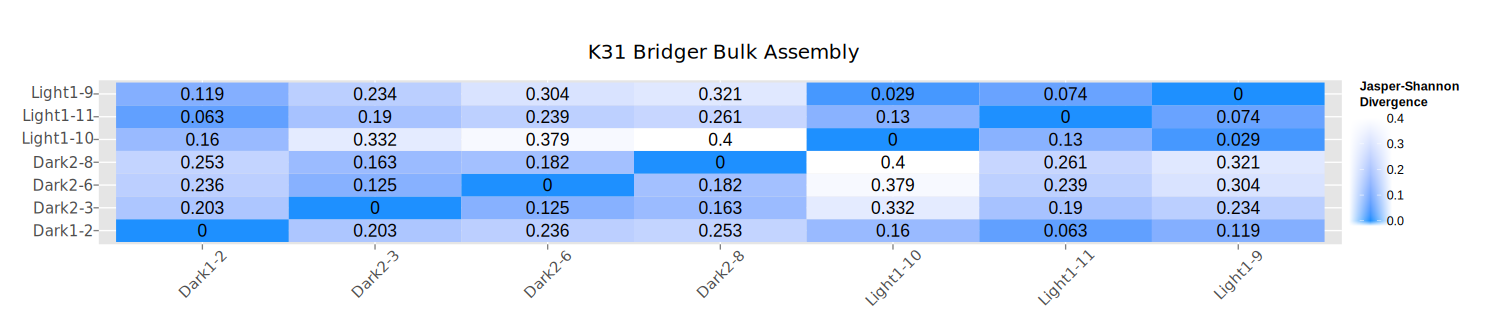
\includegraphics[width=\textwidth]{bjsvg.pdf}
    \caption[Jasper-shannon divergence of single cell transcriptome libraries]{Comparison of similarity of 
    taxonomically screened single cell libraries.  This shows how relatively divergent
each library is and demonstrates the high level of noise.  The dark and light groups
are only very faintly visible.  This further supports the use of read-mapping inferences
as qualitative rather than quantitative data for MDA-based SCT.}
\label{fig:jsd}
\end{figure}

 \begin{figure}
     \centering
     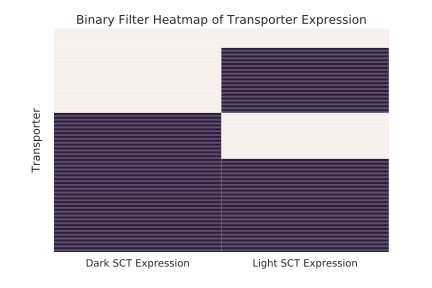
\includegraphics{transport_exp.pdf}
     \caption[Binary filter map of transporter expression between day and night]{A binary filter heatmap that displays the 4 groups of transporter
         proteins identified in the \textit{P. bursaria}-\textit{M. reisseri} 
         transcriptome.  Specifically, it shows the way that transporters
         fall into different expression ``groups'' and their relative sizes.
         In detail, 34 transporters are expressed only
         in dark single cell libraries, 48 expressed only in light libraries, the 64
         expressed in both and the 14 only recovered in the bulk libraries.}
     \label{fig:binary_expression_heatmap}
 \end{figure}


\begin{table}
    \centering

    \resizebox{\textwidth}{!}{\begin{tabular}{|c|c|c|c|}
        \hline
        \textbf{Name} & \textbf{Description/Annotation} & \textbf{Top BLASTP Hit Accession} & \textbf{Top Hit Species} \\
        \hline
        comp1093\_seq1|m.1645&Uric acid-xanthine permease& ref|XP\_005848091.1| & \textit{Chlorella variabilis} \\
        comp34246\_seq0|m.33953&Uric acid-xanthine permease & ref|XP\_005848091.1| & \textit{Chlorella variabilis}\\
        comp11781\_seq0|m.10145&Signal recognition particle protein 3 & ref|XP\_005846072.1| &  \textit{Chlorella variabilis}\\
        comp35891\_seq0|m.35196&Sensory protein & ref|WP\_027033724.1| & \textit{Mesorhizobium loti} \\
        comp13652\_seq0|m.12349&Phagocytic receptor 1b & ref|XP\_009389646.1| & \textit{Musa acuminata} \\
        comp12191\_seq1|m.10601&Inorganic phosphate transporter & ref|XP\_005852067.1| & \textit{Chlorella variabilis} \\
        comp23811\_seq0|m.24460&Inorganic pyrophosphatase & ref|WP\_028786954.1| & \textit{Terrimonas ferruginea} \\
        comp34406\_seq1|m.34111&Potassium transporter 2-like & ref|XP\_011399197.1| & \textit{Auxenochlorella protothecoides} \\
        comp25846\_seq0|m.26580&Protein trigalactosyldiacylglycerol chloroplastic & ref|XP\_005845784.1| & \textit{Chlorella variabilis}\\
        comp14064\_seq0|m.12814&Sugar transport protein 10-like & ref|XP\_005842790.1| & \textit{Chlorella variabilis} \\
        comp15360\_seq0|m.14352&Drug metabolite transporter superfamily & ref|XP\_005851889.1| & \textit{Chlorella variabilis} \\
        comp16603\_seq1|m.16010&Adenine guanine permease & ref|XP\_005850398.1| & \textit{Chlorella variabilis} \\
        comp17473\_seq0|m.17096&gpr1 fun34 family protein & ref|XP\_005848680.1 & \textit{Chlorella variabilis} \\
        comp18033\_seq0|m.17793&Hypothetical upf0065 protein & ref|WP\_019198042.1|  & \textit{Afipia birgiae} \\
        comp21389\_seq0|m.21756&Proton phosphate symporter & ref|XP\_011398136.1|& \textit{Auxenochlorella protothecoides} \\
        comp22779\_seq0|m.23394&\(Na^+\) solute transporter & ref|XP\_011396846.1| & \textit{Auxenochlorella protothecoides} \\
        comp22990\_seq0|m.23626&Inositol transporter 4-like & ref|XP\_005846641.1|  & \textit{Chlorella variabilis} \\
        comp23135\_seq0|m.23792&MFS transporter & gb|ESW58454.1| & \textit{Pseudomonas fluorescens} BBc6R8 \\
        comp26434\_seq0|m.27099&ATPase p &  ref|WP\_026773962.1|  & \textit{Sediminibacterium sp. OR43} \\
        comp26454\_seq0|m.27109&Plasma membrane iron permease & ref|XP\_005844294.1| & \textit{Chlorella variabilis} \\
        comp2716\_seq0|m.2808&Amino acid permease 6 & ref|XP\_011400870.1| & \textit{Auxenochlorella protothecoides} \\
        comp2716\_seq1|m.2811&Amino acid permease 2 & ref|XP\_011400870.1| & \textit{Auxenochlorella protothecoides} \\
        comp2716\_seq2|m.2815&Amino acid permease 2 & ref|XP\_011400870.1| & \textit{Auxenochlorella protothecoides} \\			
        comp30376\_seq0|m.30648&Amino acid permease 2 & gb|KPF41572.1| & \textit{Rhizobium} sp. AAP43 \\
        comp85197\_seq0|m.68822&Amino acid permease & ref|XP\_005846503.1| & \textit{Chlorella variabilis} \\
        comp43295\_seq0|m.41027&Lysine transporter? & ref|XP\_005847284.1| & \textit{Chlorella variabilis} \\
        comp29655\_seq0|m.30102&ABC transporter permease & ref|WP\_044404984.1| & \textit{Rhodopseudomonas palustris} \\
        comp27137\_seq0|m.27822&ABC transporter ATP-binding protein & gb|ACF01145.1| & \textit{Rhodopseudomonas palustris} TIE-1\\
        comp51985\_seq0|m.48090&ABC permease ATP-binding family protein & gb|EFD03879.1| & \textit{Propionibacterium acnes} \\
        comp13567\_seq0|m.12197&ABC transporter & ref|XP\_005849318.1| & \textit{Chlorella variabilis} \\
        comp32752\_seq0|m.32669&Membrane AAA-metalloprotease & ref|XP\_001697103.1| & \textit{Chlamydomonas reinhardtii} \\
        comp72377\_seq0|m.62224&ABC transporter permease & ref|WP\_046827962.1| & \textit{Afipia massiliensis} \\
        comp52706\_seq0|m.48773&ABC transporter permease & ref|WP\_046827962.1| & \textit{Afipia massiliensis} \\
        comp27304\_seq0|m.27991&Peptide ABC transporter permease & ref|WP\_009735611.1 & \textit{Bradyrhizobiaceae} bacterium SG-6C \\
        comp58314\_seq0|m.53037&Protein transport protein sec61 subunit alpha isoform partial & ref|XP\_005843596.1| & \textit{Chlorella variabilis} \\
        comp49211\_seq0|m.45885&ATP-binding protein & ref|WP\_051503901.1|  & \textit{Sphingomonas jaspsi} \\
        comp15817\_seq0|m.15012&Transmembrane 9 superfamily member 3 & ref|XP\_005845268.1| & \textit{Chlorella variabilis} \\
        comp39178\_seq0|m.37743&Transmembrane 9 superfamily member 3-like & ref|XP\_011395771.1| & \textit{Auxenochlorella protothecoides} \\
        comp49560\_seq0|m.46210&Transmembrane 9 superfamily member 4 & ref|XP\_005847406.1| & \textit{Chlorella variabilis} \\
        comp29161\_seq0|m.29630&Sulphate transport system & gb|AGZ19377.1| & \textit{Chlorella} sp. ArM0029B \\
        comp35923\_seq0|m.35211&Membrane protein & ref|XP\_005844583.1| & \textit{Chlorella variabilis} \\
        comp36025\_seq0|m.35298&MFS transporter & ref|WP\_012790048.1|  & \textit{Chitinophaga pinensis} \\
        comp39264\_seq0|m.37815&TctA transporteri & ref|WP\_027575203.1| & \textit{Bradyrhizobium sp. WSM1743} \\
        comp40136\_seq0|m.38461&NaDH dehydrogenase subunit 3 & ref|YP\_009049981.1| & \textit{Chlorella sorokiniana} \\
        comp40842\_seq0|m.39088&Adenine guanine permease azg1 & ref|XP\_005850398.1| & \textit{Chlorella variabilis} \\
        comp43747\_seq0|m.41450&Vesicle-associated membrane protein 726 & ref|XP\_005843431.1| & \textit{Chlorella variabilis} \\
        comp44082\_seq0|m.41788&Serine threonine protein kinase & ref|WP\_053333544.1| & \textit{Gemmatimonas phototrophica} \\
        comp44147\_seq0|m.41832&Calcium-transporting ATPase endoplasmic reticulum-type & ref|XP\_005847889.1| & \textit{Chlorella variabilis} \\
        comp45947\_seq0|m.43343&Cyclic nucleotide-binding protein & ref|XP\_005848599.1|&  \textit{Chlorella variabilis} \\
        comp46264\_seq0|m.43542&V-type proton ATPase 16 kda proteolipid subunit & ref|XP\_005848107.1| & \textit{Chlorella variabilis} \\
        comp46589\_seq0|m.43815&V-type proton ATPase subunit A3-like & ref|XP\_005849093.1| & \textit{Chlorella variabilis} \\
        comp50679\_seq0|m.47029&ER lumen protein-retaining receptor & ref|XP\_005845363.1| & \textit{Chlorella variabilis} \\
        comp51446\_seq0|m.47612&AMP-dependent synthetase & ref|WP\_019199842.1| & \textit{Afipia birgiae} \\
        comp60279\_seq0|m.54339&Presenilin-domain-containing partial & gb|KDD71768.1|  & \textit{Helicosporidium} sp. ATCC 50920\\
        comp64356\_seq0|m.57092&Zinc transporter & ref|XP\_007512557.1| & \textit{Bathycoccus prasinos} \\
        comp64706\_seq0|m.57251&ATPase P & ref|WP\_034225211.1|  & \textit{Actinotalea ferrariae} \\
        comp85939\_seq0|m.69120&Glycosyl transferase/Callose synthase & ref|XP\_011395511.1| & \textit{Auxenochlorella protothecoides} \\
        comp66975\_seq0|m.58878&Fucose permease & ref|WP\_022830286.1| & \textit{Cytophagales bacterium}  \\
    comp59167\_seq0|m.53685&Mannose-6-phosphate isomerase & ref|WP\_052557275.1|  & \textit{Gemmata} sp. IIL30 \\
        comp69839\_seq0|m.60536&Iron/manganese transporter & ref|WP\_022832831.1| & \textit{Cytophagales bacterium} B6 \\
        comp76549\_seq0|m.64487&Iron/manganese transporter & gb|AEW00627.1| & \textit{Niastella koreensis} GR20-10\\
        comp78298\_seq0|m.65658&Upf0014 membrane protein star2 & ref|WP\_035836204.1|  & \textit{Cryobacterium roopkundense} \\
        comp80077\_seq0|m.66613&Diguanylate cyclase & ref|WP\_009735916.1| & \textit{Bradyrhizobiaceae bacterium} SG-6C\\
        comp9596\_seq0|m.8023&Tricarboxylate transport membrane protein & ref|WP\_014280238.1| & \textit{Paenibacillus terrae} \\
        \hline
\end{tabular}}
    \caption[List of transporters present in both light and dark SCT libraries]{
        A complete list of the 64 putative transporters present in both Light and Dark 
    SCT libraries (at least one of each) with their annotation/description}
\end{table}

\subsection{Secreted proteins}

Using the secretome prediction consensus ensemble classifier in conservative
and permissive settings resulted in a putative secretome
of 24 and 249 proteins respectively.  Unfortunately, the permissive
group contained a significant number of transporters so the analysis
focused on the conservative consensus secreted proteins.

\begin{table}
     \resizebox{\textwidth}{!}{\begin{tabular}{|c|c|c|c|}
        \hline
        \textbf{Secreted Protein Name} & \textbf{Annotation/Description} & \textbf{Top BLASTP Hit Accession} & \textbf{Top Hit Species} \\
        \hline
        comp10940\_seq0|m.9287  &  Unknown & - & - \\ 
        comp11029\_seq0|m.9365  &  Unknown & - & - \\
        comp23584\_seq1|m.24185 &  Unknown & - & - \\
        comp13389\_seq0|m.11956 &  Unknown membrane component & ref|WP\_004718904.1| & \textit{Acinetobacter guillouiae} \\
        comp13389\_seq1|m.11962 &  Unknown membrane component & ref|WP\_004718904.1| & \textit{Acinetobacter guillouiae} \\
        comp15590\_seq0|m.14704 &  Hypothetical protein & ref|XP\_005845446.1| & \textit{Chlorella variabilis} \\
        comp19575\_seq0|m.19598 &  SOUL heme-binding protein & ref|XP\_005646909.1| & \textit{Coccomyxa subellipsoidea} \\
        comp19875\_seq0|m.19979 &  DDB1- and CUL4-associated factor 12-like & ref|XP\_005848716.1| & \textit{Chlorella variabilis} \\
        comp24544\_seq0|m.25243 &  Peptide ABC transporter substrate-binding protein & gb|KJC48675.1| & \textit{Bradyrhizobium} sp. LTSP849\\
        comp25746\_seq0|m.26477 &  Chloroplast precursor & - & - \\
        comp26585\_seq0|m.27218 &  Hypothetical protein  & ref|XP\_005846166.1| & \textit{Chlorella variabilis} \\
        comp30431\_seq0|m.30722 &  Predicted protein & - & - \\
        comp31345\_seq0|m.31491 &  Outer membrane protein & ref|WP\_008612716.1| & \textit{Joostella marina} \\
    comp41497\_seq0|m.39631 &  \(\alpha\)-l-fucosidase & ref|WP\_041886110.1| & \textit{Pedobacter} sp. NL19 \\
        comp45018\_seq0|m.42444 &  Dipeptidyle peptidase & ref|XP\_003740022.1| & \textit{Metaseiulus occidentalis} \\
        comp45978\_seq0|m.43356 &  Glycoside hydrolase & ref|WP\_049876385.1| & \textit{Sorangium cellulosus} \\
        comp48174\_seq0|m.45141 &  Recombinase & gb|AAM94959.1|  & \textit{Volvox carteri f. nagariensis} \\
        comp48206\_seq0|m.45162 &  Glutathione peroxidase & ref|WP\_022832669.1| & \textit{Cytophagales bacterium} B6 \\
        comp50890\_seq0|m.47213 &  type i polyketide synthase & ref|XP\_005650993.1| & \textit{Coccomyxa subellipsoidea} \\
    comp56156\_seq0|m.51365 &  SNase-like nuclease & gb|AIP99476.1| & \textit{Ornithobacterium rhinotracheale} ORT-UMN 88 \\
        comp57702\_seq0|m.52483 &  Unknown & - & - \\
        comp59306\_seq0|m.53753 &  soma ferritin-like & gb|AAN63032.1| & \textit{Branchiostoma lanceolatum} \\
        comp60645\_seq0|m.54526 &  Hypothetical protein & ref|XP\_005851273.1| & \textit{Chlorella variabilis} \\
    comp6932\_seq1|m.5603    & Hypothetical protein & gb|EKE16659.1| & Uncultured bacterium \\
        comp65133\_seq0|m.57547    & Raffinose synthase & ref|XP\_005845739.1| & \textit{Chlorella variabilis} \\
        \hline
\end{tabular}}
\end{table}


While many of these have no clearly defined function two of the most interesting
secreted proteins here relate to carbohydrate metabolism.
Specifically, ``comp65133\_seq0|m.57547'' which appears to be homologous 
(expectation of 1.38e-10) to Raffinose synthase, and ``comp41497\_seq0|m.42444''
which is a fucosidase. 

The secretion of a glutathione peroxidase is also intriguing.  Peroxidases
protect from oxidative damage therefore, this suggests there may be oxidative
stress within the PV lumen. 
Finally, the  membrane components could either be a misprediction and 
proteins integral to the algal outer membrane. Alternatively, they could 
be some of the hypothetical algal derived factors that integrate into the
PV membrane \citep{Kodama2009a}.


%Nitrate Reductase - m.43047  
%NADH-glutatamte reductase dehyodrgenase ?
%gluatmine synthetase ?
%No high e-value hit for Nitrite reducatase
%Ammonium transporter m.62060 in b2go not in TM pipe

\subsection{Metabolic maps}


%All prok transporters?
%One interesting aspect of comparison between the \textit{M. reisseri}
%endosymbiont and the other endosymbiotic green algae was the unique presence of 3
%additional sub-units of the branched-chain amino acid ABC transporter.
%\textit{M. reisseri} binned sequences contained the LivK, LivG, LivF sub-units
%as well as the LivH and LivM units shared by all the remaining algae. 
%This suggests either. 
%
%There are also putatively RbsB and RbsA subunits of a Ribose/D-Xylose
%ABC transporter not present in 
%and a LptB element of the ABC-2 lipopolysaccharide transporter
%and OppD oligopeptide transporter.
%
%Uracil-xanthine transporters
%
%Malate-Fumarate fumarate hydratase not present in other algae


\begin{figure}
    \includegraphics[width=\textwidth]{endo_vs_green_algae.pdf}
    \caption[KEGG maps of endosymbiont bin compared with other algae]{
    KEGG Maps contrasting endosymbiont bin with other algae. The bottom map highlights
the aspects of \textit{M. reisseri} putative transcriptome that are not present in
the other green algal species (\textit{C. variabilis} NC64A and 1N, 
and \textit{Coccomyxa subellipsoidea} C-169).}
\label{fig:algae_comp}
\end{figure}

Comparison of the \textit{M. reisseri} metabolic map against the combined
maps of the other 3 green algal datasets here (\textit{C. variabilis} 1N, 
\textit{C. variabilis} NC64A, and \textit{C. subellipsoidea}) reveals
some unique genes transcribed in \textit{M. reisseri} that are expressed while 
an endosymbiont.  

Specifically, several subunits of carotenoid biosynthesis were expressed
in \textit{M. reisseri} during endosymbiosis.  Carotenoid liposomes
have previously been implicated in the prevention of phototoxicity
in \textit{Paramecium caudatum} \citep{Rich1992}.  This means
it is possible that these carotenoids could play a role in the observed photoprotective
phenotype.
Additionally, there are numerous aspects of amino acid metabolism and degradation
only present in \textit{M. reisseri} compared to the other algal endosymbionts.
For example, lysine degradation pathway components, 
glutaminases (necessary for gluatmine, D-glutamate degradation and the metabolism of
alanine and aspartate), and urea cycle components.
Finally, there appears to be missing components of fatty acid catabolism
in \textit{M. reisseri} relative to the other endosymbionts. The degradation
products of fatty acids have been found to inhibit \textit{Chlorella} growth \citep{Ikawa1997}
meaning the partial loss of the fatty acid degradation pathways may be 
highly deleterious.  This might explain the complete loss despite the relatively
small phylogenetic distance between \textit{M. reisseri} and the other endosymbiotic
green algae.


%\begin{figure}
%    \includegraphics[width=\textwidth]{host_vs_other_host.pdf}
%    \caption[KEGG Maps of Host Bin Compared with Other \textit{Paramecium}]{
%    KEGG Maps contrasting host bin with other host}
%\end{figure}

\subsection{Metabolomics} 

\subsubsection{Global profiling}

%\begin{figure}
%    \includegraphics[width=\textwidth]{metabolome_mds.pdf}
%    \caption{Non-metric Multidimensional scaling of NBMS samples}
%    \label{fig:metabolome_nmds}
%\end{figure}
The global metabolic profiling had mixed results.
Very few metabolites were identified in the GC-QTOF
analysis and of those very few were the target carbohydrates.
Inspection of cloud plots for this dataset (\cref{fig:gcms_clouds})
indicates poor calibration of GC/MS capture parameters. 

\begin{figure}
    \centering
    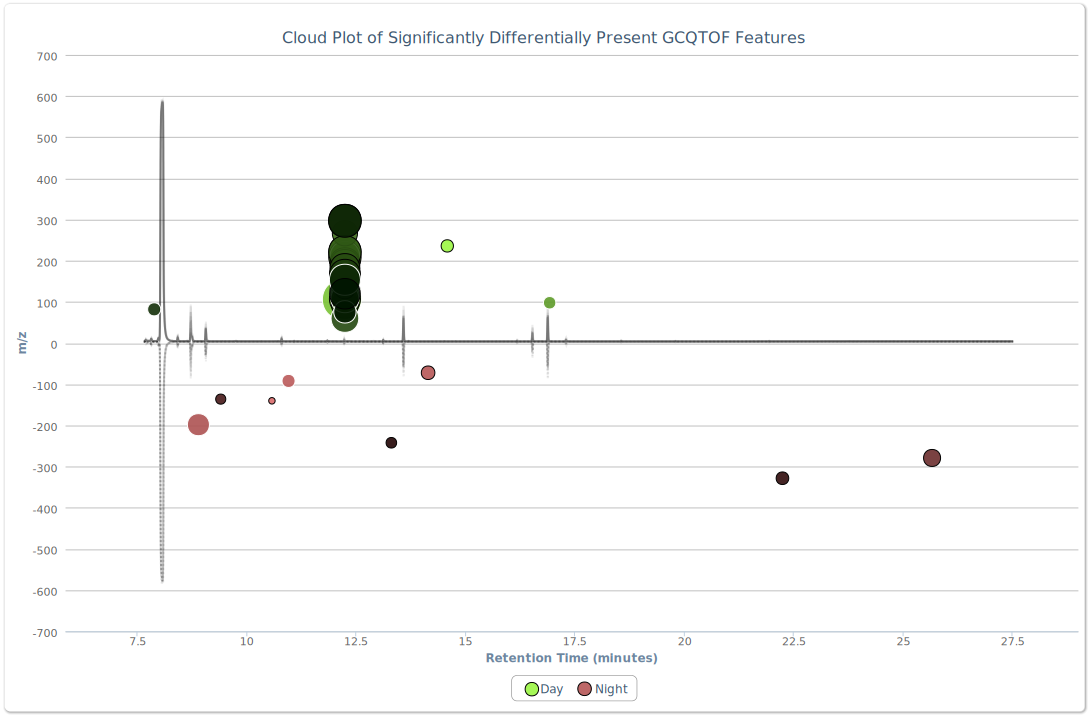
\includegraphics[width=\textwidth]{gcms_cloud_plots.pdf}
    \caption[GC-QTOF cloud plot]{Cloud plot showing for the GC-QTOF analysis. 
    The radius of a given point reflected its fold change.
    Data is filtered to those 50 points with significantly 
different expression (FDR corrected P-value of 0.01 shown by 
depth of colour).  The poor separation of components across
retention time suggests that GC could be re-calibrated to optimise
the separation of these metabolites}
    \label{fig:gcms_clouds}
\end{figure}

However, 3 carbohydrates were identified in this dataset (\cref{fig:gcms_metabolites}), including 
a putative decreased concentration of acetyl-glucose during the day.
On the other hand, a putative galactose/fructose and a fucose/galactose/rhammulose
peak demonstrated significant increases in abundance during the day with fold changes
between 3 and 4.

\begin{figure}
    \centering
    
\includegraphics{GCMS_metabolites.pdf}
    \caption[Plot of identifiable GC-QTOF metabolites]{Plot showing the
        fold change of the 23 putatively identifiable significantly
        differently present metabolites from GC-QTOF. 5 peaks
        were discarded after inspection of the EIC. 8 were discarded
    as there was no sensible annotation, 14 had no annotations.}
    \label{fig:gcms_metabolites}
\end{figure}

LC-QTOF seemed to be more calibrated - identifying a much greater number of metabolites
(\cref{fig:posqtofdown}, \cref{fig:posqtofup}, \cref{fig:negqtof})
with better separation (\cref{fig:lcms_clouds}).

\begin{figure}
    \centering
    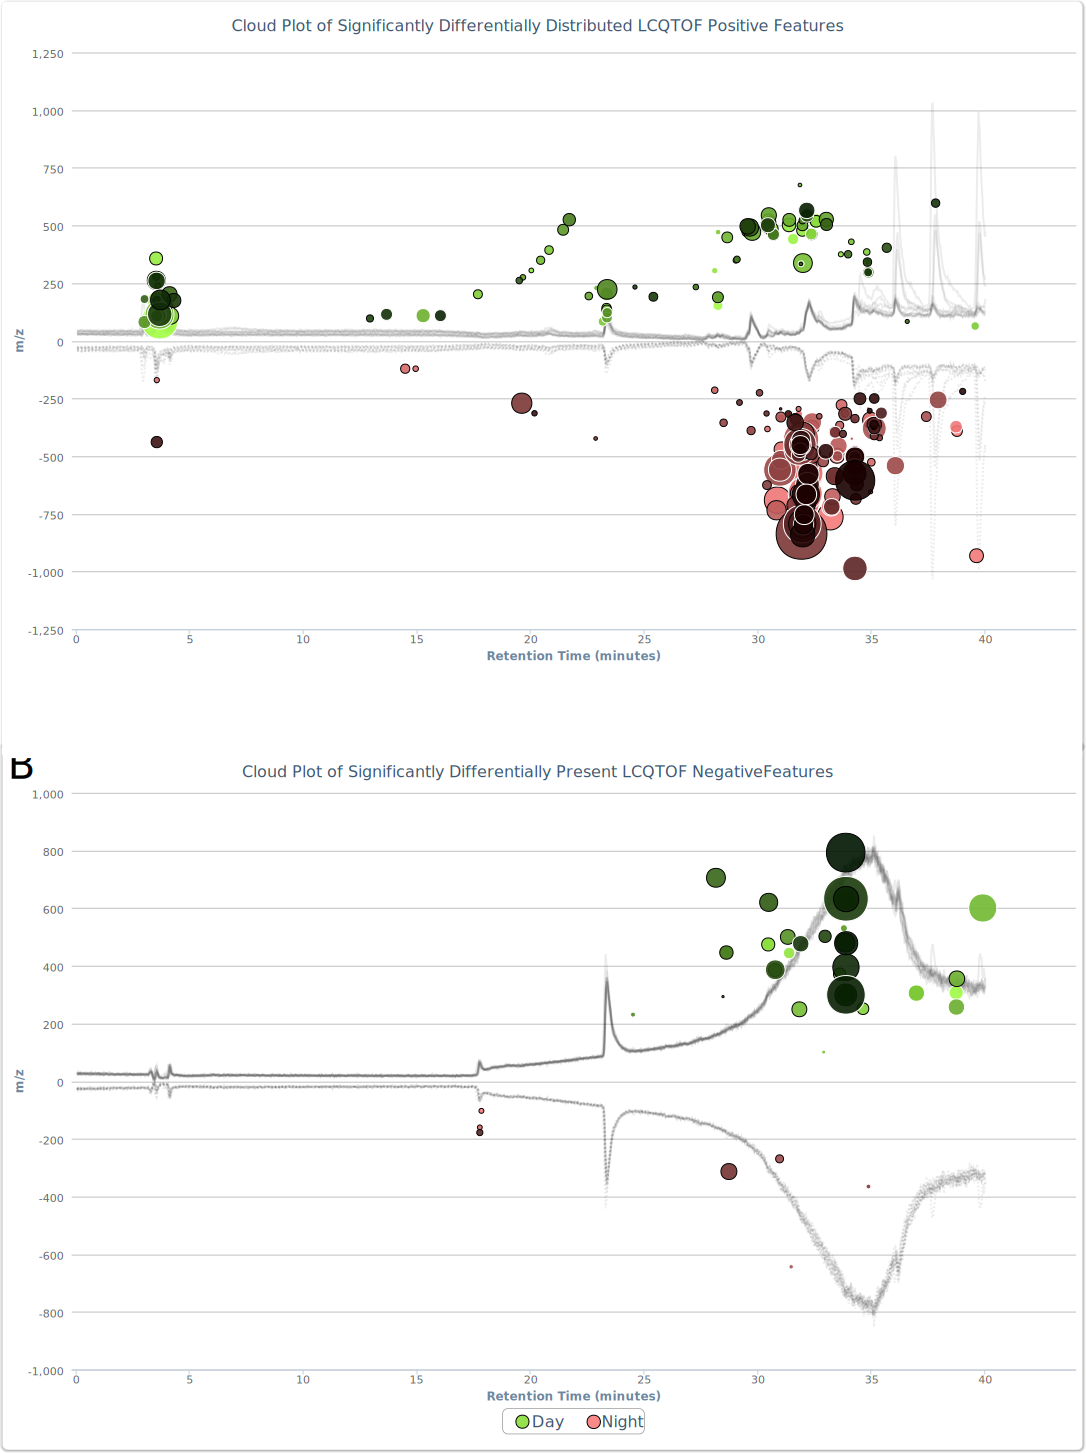
\includegraphics[width=\textwidth]{lcms_cloud_plots.pdf}
    \caption[LC-QTOF cloud plots]{LC-QTOF cloud plots with \textbf{A} showing
        the positive polarity analysis and \textbf{B} showing the negative polarity. 
        The radius
        of a given point represents its fold change, with larger
        radius indicating a larger fold change.   Data is filtered 
        only to include points with significantly different expression
        and the depth of colour indicates the P-value.   Contrary to
        the GC-QTOF analysis LC-QTOF shows a relatively good
        separation of metabolites.  This plot also
    emphasises that far more metabolites were detected and discovered
differentially expressed under positive ionisation.}
    \label{fig:lcms_clouds}
\end{figure}


\begin{figure}
    \centering
    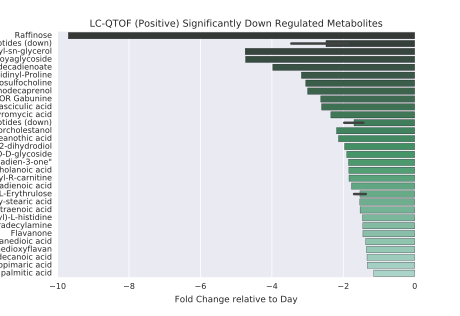
\includegraphics[width=\textwidth]{LCMS_pos_down_metabolites.pdf}
    \caption[LC-QTOF positive ionisation lowered concentration metabolites]{LC-QTOF positive ionisation detected metabolites
        that were significantly more abundant at night relative to the day. Of the 254 positive significantly different present metabolites,
        19 were removed after manual inspection of peaks, 95 were removed due to having no METLIN hits.}
    \label{fig:posqtofdown}
\end{figure}


\begin{figure}
    \centering
    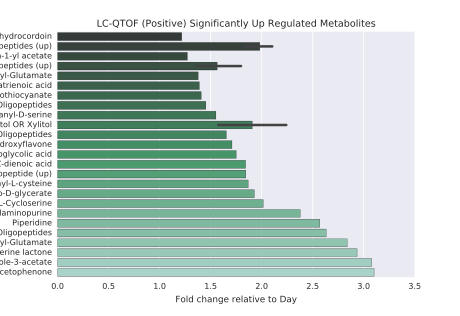
\includegraphics[width=\textwidth]{LCMS_pos_up_metabolites.pdf}
    \caption[LC-QTOF positive ionisation increased concentration metabolites]{LC-QTOF positive ionisation detected metabolites
        that were significantly more abundant in the day relative to night. 254 positive significantly different present metabolites,
        19 were removed after manual inspection of peaks, 95 were removed due to having no METLIN hits.}
    \label{fig:posqtofup}
\end{figure}


\begin{figure}
    \centering
    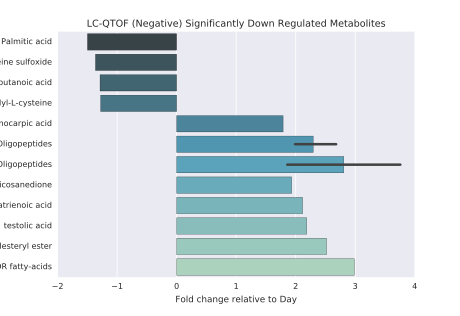
\includegraphics[width=\textwidth]{LCMS_neg_metabolites.pdf}
    \caption[LC-QTOF negative ionisation metabolites]{LC-QTOF negative ionisation metabolites identified
        as significantly higher or lower concentration between day and night. 
        43 significantly different present metabolites were identified,
        3 were removed after manual inspection of peaks, 17 were removed due
    to having no METLIN hits.}
    \label{fig:negqtof}
\end{figure}


Several amino acids and oligopeptides were identified as having significantly
different day/night concentrations in the LC-QTOF analyses. However,
the most significant peaks were that of a hugely decreased abundance of
Raffinose (fold change of 9.7) during the day.  
On the other hand, the polyols Arabitol/Xylitol were present at higher quantities (1.52-2.24 fold)
and arabinose (2.7 fold) during lit conditions.
%inositol transporter comp22990\_seq0|m.23526
%
%Xylitol or arabinose likely play a role
%Arabinose is likely to play a role with the signficant (2.7) fold up-regulation
%of arabinosyl glucoside in LC-QTOF pos,
%Arabitol/Xylitol of 1.52 and 2.24 
%In GCMS Arabionic acid/xylonate 3.1 up 
%
%fucose permease comp66975\_seq0|m.58878


\subsubsection{Targeted amino acid analysis}

\begin{figure}
    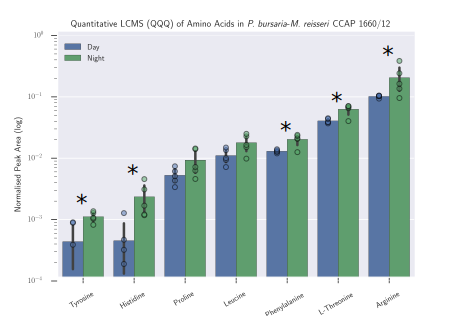
\includegraphics[width=\textwidth]{AA_LCMS.pdf}
    \caption[LC-QQQ quantitative analysis of amino acids]{LC-QQQ analysis
        of amino acid abundances. Normalised Peak Areas 
        Calibration was conducted using Day1 and Night1 samples at two titrations, as well as Asn-Gln-Tryptamine and Sigma AA mixes.
    Calibration and quantitative analysis failed for the following amino acids: 
Glutamic Acid, Tryptamine, Asparagine, Tryptophan, Isoleucine, Methionine, Valine, Serine, Glutamate, Glutamine, Aspartic acid, Cysteine or Lysine.
    Significant concentration differences between day and night (as determined via Welch's `\textit{t}' are indicated by an asterisk).}
    \label{fig:amino_acids}
\end{figure}

The targeted quantitative analysis of the amino acids in the system
between day and night also had mixed results.  The majority of amino
acids were not reliably recovered and calibration curves could not be fitted.
Therefore, several key amino acids remain unprofiled.
The relatively large concentration of arginine as well as significant
day-night differences suggests that this may be an important nitrogen
source for \textit{M. reisseri} during endosymbiosis.


\section{Discussion}

\subsection{Novel sugars implicated in the endosymbiosis}

One of the key findings supported by multiple lines of evidence
is the existence of roles for sugars not previously implicated in the
function of \textit{P. bursaria} - green algal endosymbioses. 
Specifically, arabinose, raffinose and fucose. 

Fucose is identified as having a significantly higher concentration during the day 
and the endosymbiont expresses a fucose permease in both lit and dark conditions.
Arabinose is similarly significantly at greater abundance the day 
however, no arabinose transporter was directly identified in the endosymbiont 
transcriptome.  It is possible that one of the MFS group transporter identified is 
capable of uptake of this compound though. 

Raffinose was both detected
at significantly lower abundance during the day in the metabolomics 
and a raffinose synthase predicted as a secreted protein.
An uptake transporter for raffinose was not identified in the endosymbiont 
but again it is possible that one of the MFS transporter may be capable
of the uptake of this compound.  Alternatively, the host could encode
a transporter for raffinose uptake into the host cytoplasm.
A transporter that was directly identified in the endosymbiont was that for inositol.
As raffinose synthase function involves the production of inositol and raffinose
from galactinol and sucrose \citep{Caspi2007} this suggests that inositol
is either taken up by the endosymbiont or pumped into the PV lumen.

It seems clear that raffinose plays some significant role in the endosymbiosis
especially as it is likely to be synthesised within the PV lumen itself due
to the putatively secreted peptide.
Raffinose has been associated with cold shock in
\textit{Parachlorella kessleri} (formerly \textit{C. vulgaris}),
accumulating during cold exposure and disappearing after returning
to normal temperatures.
Specifically, it has also been directly associated
with cryoprotection of thykaloid membranes \citep{Lineberger1980}.
Raffinose and another Raffinose Family Oligosaccharide (RFO) 
stachyose are also generated in gymnopserms during
the cold season \citep{Kandler1982}.
Interestingly, raffinose has been found to inhibit growth under
isosomotic conditions in a \textit{C. vulgaris} 
\citep{Setter1979}.

Therefore, it is not immediately clear what role raffinose may play in the endosymbiosis. 
I present 2 hypotheses: firstly, that it may be involved in the stability
and maintenance of the PV membrane due to its previously implicated
role in cryoprotection of thykaloid membranes and secondly, that it may form a way
in which the endosymbiont can ``sequester'' released carbohydrates 
from the host by converting them to a format the \textit{P. bursaria} host
cannot uptake.  
This doesn't directly explain 
the significantly high concentration
of raffinose at night relative to day, however, 
this could relate to the storage of photosynthate in the
form of raffinose in the absence
of active photosynthesis.

It is worth noting that the identification of other secreted
proteins related to the hypothetical synthesis and metabolism 
of complex sugars in the PV could have been missed due to 
poor terminal resolution of transcripts during sequencing.
This is particularly problematic for bulk RNAseq and 
low terminal coverage and thus less trust-worthy data 
was identified in a preliminary analysis of this type 
of transcriptomic data.  Theoretically,
due to the ligation step, MDA based sc-RNAseq shouldn't
have this issue.  However, it seems likely the general
noise and biases of MDA may have rendered a reduced
positional bias as a moot issue.

%may support this, assuming a constant
%level of raffinose synthase but a supply of photosynthate pre-cursors (maltose, 
%glucose and/or fructose) that is limited to just lit conditions then 
%the raffinose concentration may increase gradually 

\subsection{Alternative exchanged amino acids in \textit{P. bursaria}-\textit{M. reisseri}}

The failure of accurate quantification in the second round
of LC-QQQ spectrometry for the majority of amino acids 
is problematic.  However, this targeted approach still revealed
useful information regarding the relative abundance of certain amino acids.

Particularly, both the high concentration of arginine as well
as its significantly differential abundance between day and night
indicates that this amino acid may well form a major component of 
host provided nitrogen for \textit{M. reisseri}. This is in
concordance with previous findings suggesting 
the importance of this amino acid in the \textit{C. variabilis}
endosymbiosis \citep{Kato2006}.  The presence of elements of 
arginine metabolism pathways such as the urea cycle in the transcriptome 
also supports this hypothesis. 


Despite not have been implicated in previous analyses
as one of the key amino acid nitrogen sources, the identification
of both high quantities and differential abundance of
threonine and phenylalanine suggests that these
amino acids may play a role in the host-endosymbiont
barter system of \textit{P. bursaria}-\textit{M. reisseri}.
Additionally, the unique presence of lysine, glutamine and D-glutamate 
degradation pathways in \textit{M. reisseri} relative to other green algae
suggests that these amino acids also comprise an element of the host-derived
nitrogen supply.
The differential abundances of the amino acids as well as
differential numbers of reads mapping to putative amino acid
transporters indicates a potential light-dependent amino acid
uptake mechanism in the endosymbiont.


This markedly different behaviour in \textit{M. reisseri} relative
to the other algal endosymbionts suggests that the feeding experiment
results by \citep{Kato2006} and \citep{Kato2009a} need 
to be re-evaluated for \textit{M. reisseri}. This also
adds further evidence of a broad diversity of endosymbiotic
relationships and traits among the various algal endosymbioses
of \textit{P. bursaria}.


Unfortunately, a failure to accurately quantify and calibrate
for several amino acids means this targeted metabolomic analysis
is incomplete.  Of particular interest, is the remaining 5 amino acids
implicated in \textit{C. variabilis} F36-ZK's endosymbiosis.


There is also a potential supply of oligopeptides to the endosymbiont.
This is evidenced by the presence of a partial oligopeptide transporter 
combined with the observed high concentrations of various 3- and 4-mer oligopeptides.
Previous studies focusing exclusively on endosymbiont utilisation
and uptake of individual amino acids (e.g. those reviewed in \citep{Kato2009a}) 
may have missed on the role of these in host-endosymbiont nitrogen flux.
This, therefore, merits further analysis.



%There is reason to believe that \textit{M. reisseri} CCAP 1660/12
%endosymbiont displays a similar system to that of the Japanese
%\textit{C. variabilis} F36-ZK strain in terms of amino acid usage. 
%
%Intriguingly, the transcriptome reveals the presence of all sub-units
%of the ABC-type branched amino-acid transporter not present in 
%the other endosymbiotic green algae. However, the non-differential
%abundance of Leucine makes it hard to determine.
%

In terms of other nitrogen sources, i.e. nitrate and nitrite:
NR and NiR are both present in the \textit{M. reisseri} binned transcriptome.
This supports findings that \textit{M. reisseri} can utilise nitrate and nitrite.
However, it is possible that these enzymes are non-functional such as the mutants
present in \textit{C. variabilis} NC64A and F36-ZK.


\subsection{Potentially missing transporters and secreted proteins}

The identification and analysis of secreted and transporter proteins,
as well as the metabolic mapping are fundamentally reliant on the quality and completion
of the host and endosymbiont binned transcriptomes. 
Transcripts may be missing from these bins either due to failure to assemble, 
cryptic MDA biases, or erroneous binning into bins other than host or endosymbiont.

It is a cause for concern that there are a number of endosymbiont secreted and transporter proteins 
which have top BLASTP hits against bacterial species.  
On inspection many of these do have
other hits to green algal species at slightly lower expectation
therefore binning could be working as intended. However,
bacterial contamination of the endosymbiont bin is 
a very real possibility. 
Further studies should confirm the identity of these proteins using
manual in-depth phylogenetics instead of the high-throughput and potentially
error prone method used in transcript binning.


There is evidence that binned endosymbiont transcriptomes are incomplete in the large
disparity in predicted transporter set sizes between the genomes and transcriptome
based datasets.  However,
we are not necessarily interested in all the transporters and secreted proteins
that the endosymbiont is capable of producing but merely those that it is producing
while an endosymbiont. 
A high level of transcription as an endosymbiont
suggests that the function of given protein plays a significant role in symbiosis.
Therefore, theoretically the only major group of factors that are both
involved in endosymbiosis and systematically absent from these binned
transcripts are those of effectors related to the establishment of endosymbiosis
that are not expressed during the rest of the endosymbiotic relationship.


One set of proteins in which erroneous binning may be particularly
problematic is that of proteins which have recently undergone endosymbiotic
gene transfer (EGT) between endosymbiont and host \citep{Timmis2004} or that have been horizontally
acquired from other sources.  In the former case,
this is well observed phenomenon that has resulted in the eventual loss
of the endosymbiont in the majority of algal secondary endosymbiotic organelles
as genes are transferred to the host nucleus
\citep{Keeling2008a,Archibald2005,Timmis2004,Keeling2004a}.
It is unknown and difficult to determine to what extent the 
unusual nuclear dimorphism and germline sequestration of the host 
will effect this form of transfer. However, hypothetically this should
present a barrier to such transfers. 
As some \textit{M. reisseri} and \textit{Chlorella} endosymbionts 
have been demonstrated as capable of free-living and metabolic
co-dependence has putatively not become fixed it is 
unlikely that EGT has occurred between host and endosymbiont as extensively
as that observed in established photosynthetic organelles. 
Fortunately, the binning method used means that while some peptides
may have been falsely assigned to wrong bin, all ``host'' and
``endosymbiont'' ORFs that were either so novel they lacked
any homology to known proteins or were recently acquired from
bacteria were still included in this analysis, just not necessarily
attributed to the correct partner.

As for the latter case of HGT from other sources, this will lead to the misclassification
of proteins into the ``food'' or ``unknown'' bin and thus their discard. 
This is potentially problematic as there is evidence for bacterially acquired 
hexose-phosphate transporters playing a key role in the 
establishment of primary plastid endosymbiosis \citep{Price2012,Karkar2015a}.
There is also evidence of the acquisition of a bacterial polyamine
biosynthesis pathway within the host \textit{Paramecium} \citep{Li2015b}.


Ideally, future work could expand the component analyses over the 
``unknown'' and ``food'' binned sequences in combination with synteny
analyses using genomic sequences to investigate and identify
potential horizontally acquired transporters that may play a role.

Another issue with the binning approach used is the possibility
of totally novel transporter (and other proteins) not being classified
due to the dependence of the binning on homology to known sequences.
Therefore, totally novel proteins would not have been identified as 
``host'' or ``endosymbiont''.  Unfortunately, this problem 
could only properly be resolved with a 
genome sequence for both host and endosymbiont which was outside
the scope of this analysis. 

Finally, there are two additional difficulties specific to transporter and secretome prediction.
In terms of secreted proteins, without knowledge of \textit{P. bursaria}'s intracellular trafficking
system it is not possible to easily infer which host peptides are secreted into
the PV.  For this reason, analysis of secreted proteins focused on 
the endosymbiont bin as the secretion signal are generally better conserved
and established. 

In the case of transporters the risk of false positives where sensors are 
misidentified as transporters is fairly high. 
Only a minimal (as few as
a single amino acid) divergence is sufficient to convert a transporter protein 
to non-transporting sensor proteins \citep{Lalonde1999,Bianchi2010}.
However, sensor proteins are likely to play important roles in the function
of this endosymbiosis so accidental identification may not be a major issue but
it does mean transporter activity needs to be verified for all predictions.


Prediction methods used to identify
transporter and secreted proteins 
could also be further improved by more careful 
application of state-of-the-art classification
algorithms. 
Prediction of protein secretion could be improved
using recent approaches such as recursive
neural network models like long-short term memory networks 
\citep{Hochreiter1997,Greff2015}.
These are well suited to arbitrary length sequence data so wouldn't 
require work-arounds to accommodate variable length signal 
peptides.  They are also capable of representation learning
so the identification of sequence features that best
predict localisation would be unnecessary. 
Alternatively, existing prediction tools could be combined
in a more sophisticated way than the conservative consensus
ensemble used in this analysis.  For example,
the various predictors could be combined using Bayesian
model combination \citep{Monteith2011}.


However, even with these improved predictions, it is still 
best to consider all analyses
of these transcriptomes as proof of presence but not proof of absence
of any component. Furthermore, any identified protein should be validated
individually using immunolocalisation and (q)PCR based analyses.

\subsection{Metabolomics shows promise}

The pilot application of metabolomics demonstrated mixed results.
There was poor performance of GC/MS with a failure to
comprehensively profile carbohydrates. Several 
compounds strongly implicated in the endosymbiosis
were not detected e.g. maltose, and glucose.  This was potentially
due to the miscalibration of gas chromatography leading to poor 
separation of components. 

While LC/MS analyses did prove relatively successful, a careful
validation of metabolites of interest using multi-reaction monitoring
and tandem spectrometry would be necessary to make firm predictions.
Additionally, advanced novel techniques such as nanoscale 
secondary ion mass spectrometry combined with 
microscopy and isotope labelling could theoretically allow direct analysis 
of metabolites present in the PV \citep{Kopp2015,Legin2014}.

The targeted quantitative LC/MS of amino acids needs further optimisation
and re-running due to the inability to fit calibration curves to the majority
of amino acids. Despite this, the technique did prove effective at identifying 
a potential role for several amino acids not previously implicated in this
endosymbiosis.

Finally, one more improvement to the metabolomics analyses 
would include more advanced hypothesis testing than the 
corrected unequal variance \(t\)-test used e.g.
Kurschke's Bayesian BEST algorithm \citep{Kruschke2013}.
This has the advantage of a Bayesian inference which can be 
made robust to multiple comparisons without need for extensive correction
procedures via standard multi-level approaches \citep{Gelman2009}.


\section{Conclusion}

This analysis of host-endosymbiont metabolic integration 
has lead to some promising results.
Namely, discovering quantitative data supporting the mechanism by which
the host likely provides a nitrogen source to the endosymbiont. 
Specifically, a novel group of amino acids may well be used in 
\textit{M. reisseri} endosymbiosis: lysine, d-glutamate, 
threonine, and phenylalanine, as well as the previously implicated
arginine and glutamine \citep{Kato2009a}.  Additionally,
potential novel roles for carbohydrates previously
not associated with \textit{P. bursaria} endosymbioses, specifically
fucose, arabinose and raffinose have been identified. 
Unfortunately, poor resolution and identification of carbohydrates 
in GC/QTOF prevents a thorough analysis of endosymbiotic carbohydrate
metabolism. 
Finally, \textit{M. reisseri} appears not to express elements of fatty
acid degradation present in the other algal endosymbionts. 
This is potentially interesting as fatty acid metabolism has previously
been identified as a key conserved function of plastids \citep{Donaher2009}.
However, further work is needed to confirm both the role and localisation of
these compounds and their facilitators.


Ultimately, the key finding from this analysis
is that \textit{M. reisseri} exhibit a range of adaptations
to endosymbiosis that are distinct from previously
studied algal strains such as \textit{C. variabilis}.


%mycosporina amino acids - shikimate pathway - protect agains UVR \citep{Sommaruga2009} (Shick and dunlap 2002)
%chlorella made MAA found in cilliates sonntag2007 
%Negative in p bursaria chlorella thoufgh summerer2009
